
%%%%%%%%%%%%%%%%%%%%%%%%%%%%%%%%%%%%%%%%%%%%%%%%%%%%%%%%%%%%%%%%%%%%%%%%%%
%%%%%%%%%%%%   CHAPTER 2   %%%%%%%%%%%%%%%%%%%%%%%%%%%%%%%%%%%%%%%%%%%%%%%%
%%%%%%%%%%%%%%%%%%%%%%%%%%%%%%%%%%%%%%%%%%%%%%%%%%%%%%%%%%%%%%%%%%%%%%%%%%
\chapter{Background and Related work}
\label{chap:backgroundandrelatedwork}

%intro
%
This chapter initially discusses the background of Stereo vision, implementation platforms, Nema eGPU architecture, and kernel \& mapping information of the eGPU. Towards the end, current research done on the Stereo vision and GPU fields are discussed along with implication of their importance.


%%%%%%%%%%%%%%%%%%%%%%%%%%%%%%%%%%%%%
%%%%%%%%%%%%%%%%%%%%%%%%%%%%%%%%%%%%%
%%%%%%%%%%%%   SECTION   %%%%%%%%%%%%
%%%%%%%%%%%%%%%%%%%%%%%%%%%%%%%%%%%%%
%%%%%%%%%%%%%%%%%%%%%%%%%%%%%%%%%%%%%
\section{Stereo vision}
\label{s:stereovision}

Stereo vision involves extraction of depth information from multiple camera images of the same scene. The basic form of Stereo vision is binocular Stereo vision involving two cameras as shown in the Figure \ref{fig:bsv}. In the figure, it can be noticed that both the Left and the Right camera, take the image of a point P. These two cameras are separated by a distance b, called the baseline. The image planes of both the cameras are also shown in the figure. These image planes contain the pixel projections of the points in the scene for each of the cameras respectively. For example, the right camera sees the point P on the pixel U\textsubscript{R}, while the left camera sees the point P in the pixel U\textsubscript{L}. It can be seen that there is a shift along the X-axis while comparing the projections of the point in the two image planes. That is, in the above figure pixel U\textsubscript{R} is closer to the left end of the image plane while the pixel U\textsubscript{L} is closer to the right end.  This shift increases as the point P gets closer to the camera. Thus, if one can measure the shift in the position of the pixel for any point in the scene between the two image planes, the relative depth (disparity) of that point in the scene can be found out. An image giving disparity of all the points in the image plane is called disparity map (DM). The absolute depth can also be calculated if the focal lengths of the cameras are known.\\


\begin{figure}[!htbp]
    \center
    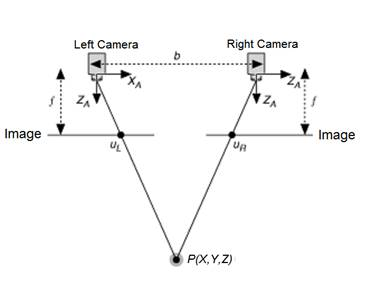
\includegraphics{figures/StereoVision}
    \caption{Illustration of binocular stereovision \cite{_3d_2013}.}
    \label{fig:bsv}
\end{figure}

This thesis deals with binocular Stereo vision (Stereo vision involving two cameras). In binocular Stereo vision, image from one of the cameras is taken. Then for each pixel in that image, the pixel corresponding to the same point in the scene is found in the image from the other camera. Then the positions of the two pixels in their respective image planes are compared in order to arrive at the depth of the point in the scene. In order to arrive at the depth, the cameras' geometry and properties need to be taken into account\\

\begin{figure}[!htbp]
    \center
    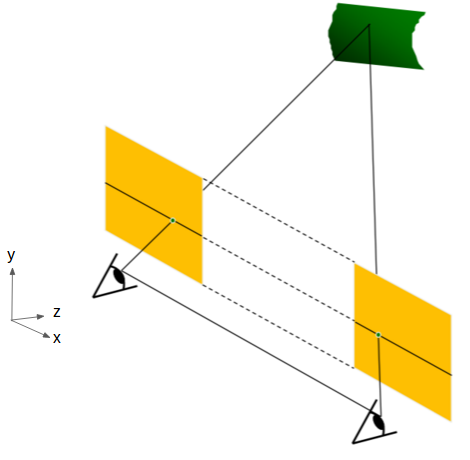
\includegraphics[width=75mm]{figures/Assumptions}
    \caption{Assumptions on stereovision set up \cite{derek_hoiem_epipolar_2011}.}
    \label{fig:assumptionssv}
\end{figure}

There are some assumptions made regarding the stereo images used in this thesis:
\begin{enumerate}
    \item The left and the right cameras used to take the images are synchronous i.e. the images from the left and the right cameras are taken at the same instant. This is in contrast with another method where a single camera takes image of a scene from multiple points at different instances of time.
    \item The image planes of the cameras used in taking images are coplanar.
    \item The reference axes of the image planes coincide.
    \item The centers of the cameras used to take the images are  in same height. The points 2,3 and 4 together imply that the image planes of the right and left cameras have the same reference axes x,y, and z and they are only shifted laterally along the x-axis (they are not rotated).
    \item The physical properties of the cameras, for example focal length and the resolution are the same.
\end{enumerate}

Samples of images used in this thesis complying with the given conditions are shown in the Figure \ref{fig:samplessv}.

\begin{figure}[!htbp]
\begin{subfigure}{.5\textwidth}
  \centering
  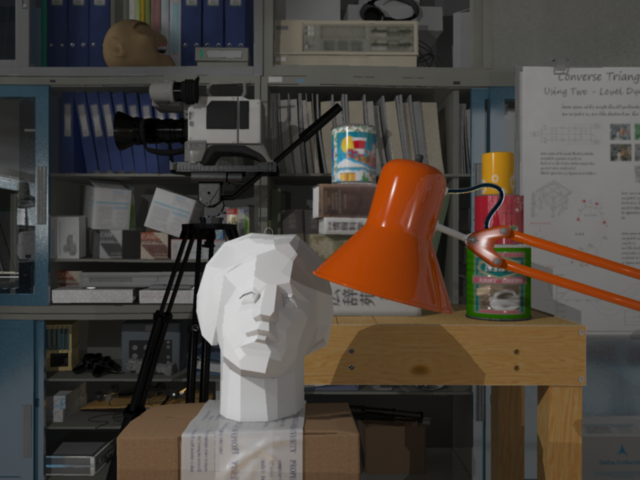
\includegraphics[width=.8\linewidth]{figures/frame_1_left}
  \caption{Tsukuba left}
  \label{fig:sfig1}
\end{subfigure}%
\begin{subfigure}{.5\textwidth}
  \centering
  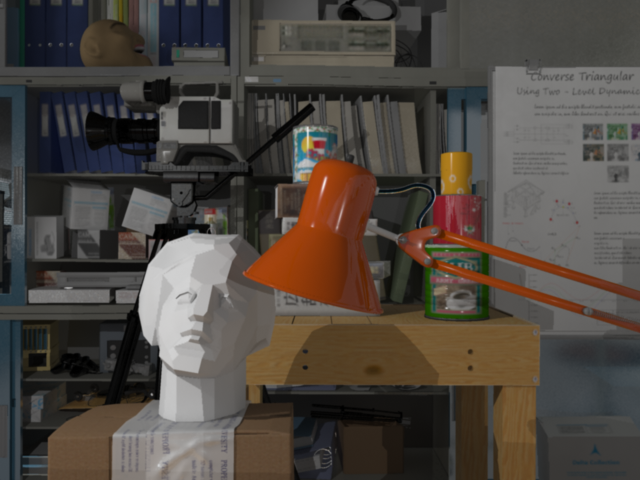
\includegraphics[width=.8\linewidth]{figures/frame_1_right}
  \caption{Tsukuba right}
  \label{fig:sfig2}
\end{subfigure}
\begin{subfigure}{.5\textwidth}
  \centering
  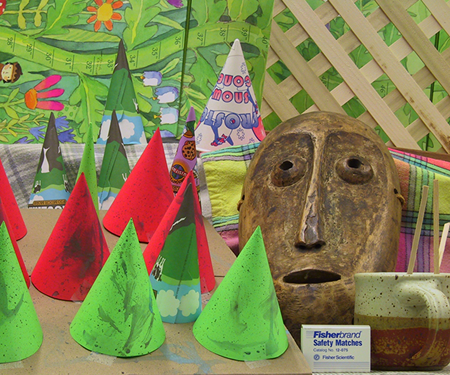
\includegraphics[width=.8\linewidth]{figures/ConeL}
  \caption{Middlebury left}
  \label{fig:sfig3}
\end{subfigure}%
\begin{subfigure}{.5\textwidth}
  \centering
  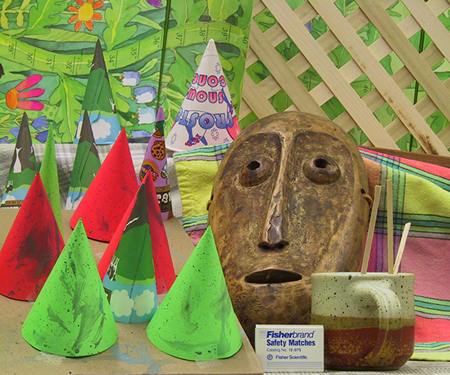
\includegraphics[width=.8\linewidth]{figures/ConeR}
  \caption{Middlebury right}
  \label{fig:sfig4}
\end{subfigure}
\begin{subfigure}{.5\textwidth}
  \centering
  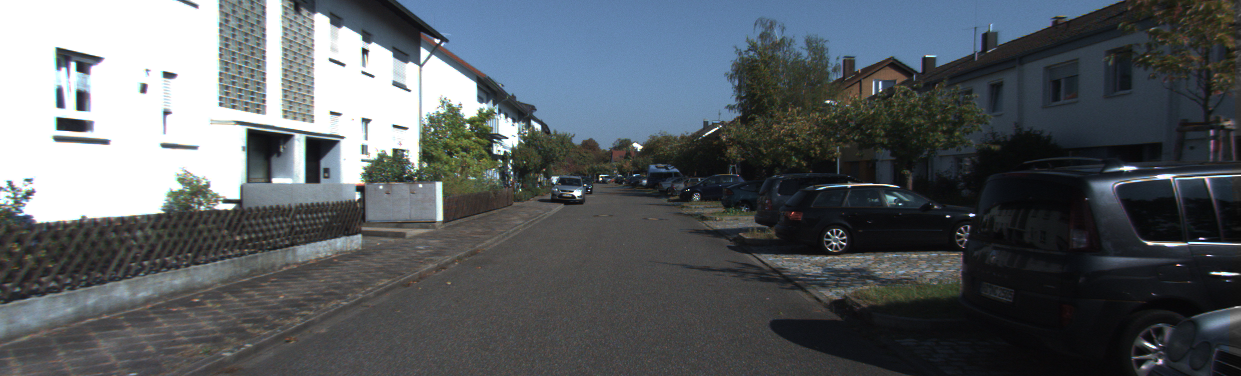
\includegraphics[width=.8\linewidth]{figures/RoadL}
  \caption{KIT left}
  \label{fig:sfig5}
\end{subfigure}%
\begin{subfigure}{.5\textwidth}
  \centering
  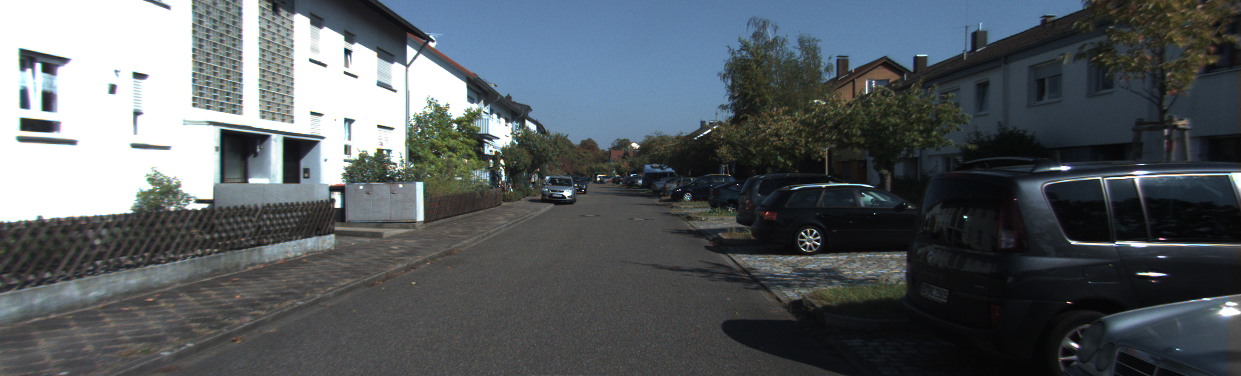
\includegraphics[width=.8\linewidth]{figures/RoadR}
  \caption{KIT right}
  \label{fig:sfig6}
\end{subfigure}
\caption{Sample Stereo vision images}
\label{fig:samplessv}
\end{figure}

%%%%%%%%%%%%%%%%%%%%%%%%%
%%%%%   SUB-SECTION   %%%
%%%%%%%%%%%%%%%%%%%%%%%%%
%%%%%%%%%%%%%%%%%%%%%%%%%
\subsection{Disparity Map evaluation}
\label{s:stereovision:bmpre}

The quality of the DM obtained by an algorithm is decided by its comparison with the ground truth. There are many methods of error estimation of a DM with respect to ground truth. In this thesis, Bad Matched Pixels Relative Error (BMPRE) method proposed by Cabezas et al. \cite{Cabezas2012} is used for the error estimation and hence the functional verification of the algorithm across parameters. With the ground truth available, the relative error of each pixel with respect to the true disparity value sheds light on how good the algorithm's performance is in estimating the depth values. The BMPRE method considers these aspects during the error evaluation and is hence chosen.

The BMPRE measure is formulated as:

\begin{equation}
 BMPRE =\sum\nolimits_{(x,y)}^{N}
   \begin{cases}
    \tau(x,y)       & \quad \text{if } \Delta({\rm x}, {\rm y}) > \delta\\
    0  & \quad \text{if } \Delta({\rm x}, {\rm y})\leq \delta\\
  \end{cases}
  \label{eqn:bmpre}
\end{equation}

where $\Delta(x,y)$ is the absolute difference between the obtained disparity and the ground truth at coordinates (x,y) $\delta$ is the threshold for error and $\tau(x,y)$ is given by:
\[
  \tau({\rm x}, {\rm y})=
  \begin{cases}
    \Delta(x,y)\over {D}_{true}(x,y)       & \quad \text{if } {D}_{true}(x,y) > 0\\
    0  & \quad \text{if } \text{otherwise}\\
  \end{cases}
\]

Here ${D}_{true}(x,y)$ indicates the disparity value of the ground truth at position (x,y). In the current thesis $\delta$ value of 2 is chosen for the calculation. The choice of $\delta$ is arbitrary as the performace of same algorithm across parameters is compared.

%%%%%%%%%%%%%%%%%%%%%%%%%%%%%%%%%%%%%
%%%%%%%%%%%%%%%%%%%%%%%%%%%%%%%%%%%%%
%%%%%%%%%%%%   SECTION   %%%%%%%%%%%%
%%%%%%%%%%%%%%%%%%%%%%%%%%%%%%%%%%%%%
%%%%%%%%%%%%%%%%%%%%%%%%%%%%%%%%%%%%%
\section{GPU hardware}
\label{s:gpuhw}

%
The ALUs in GPU are simpler in nature compared to those in CPUs. A particular ALU in a GPU takes more time for execution of a single instruction compared to an ALU in a CPU. Thus, CPU is said to be latency optimised compared to GPU. However, GPUs have a huge number of ALUs for each core (or multiprocessor) compared to CPUs. This means that all the ALUs can work at the same time thus increasing the throughput. Overall, this makes the GPU much faster for parallelizable problems. CPUs are low latency low throughput devices while GPUs are high latency high throughput devices. The architecture of GPU in comparison with CPU is as shown in the Figure \ref{fig:cpugpu}.

\begin{figure}
    \center
    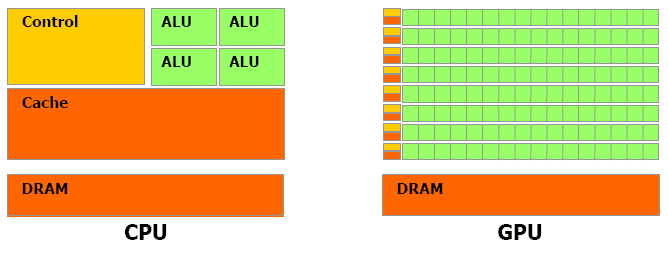
\includegraphics[width=.8\linewidth]{figures/cpugpu}
    \caption{Architecture comparison between CPU and GPU \cite{gpu2008}.}
    \label{fig:cpugpu}
\end{figure}


%%%%%%%%%%%%%%%%%%%%%%%%%
%%%%%   SUB-SECTION   %%%
%%%%%%%%%%%%%%%%%%%%%%%%%
%%%%%%%%%%%%%%%%%%%%%%%%%
\subsection{Nema hardware}
\label{s:gpuhw:nema}

Nema is an embedded GPU platform designed by ThinkSilicon taking low energy consumption and silicon footprint into consideration \cite{_nema|s}. It is scalable many-core, multi-threaded design with both graphics rendering and general computing capabilities. It is deployed in a reusable soft IP core suitable for ASIC or FPGA implementation. Nema GPU employs multiple processing cores in clusters, and multiple clusters can be connected via a proprietary network-on-chip (NoC). This along with a memory subsystem design allows Nema to be scaled to a multi-core GPU of a size required by the problem in hand. Software development for Nema can be done through industry-standard APIs supported by a dedicated LLVM/Clang compiler toolchain which adapts to the changing architecture. Nema currently supports C/C++ programming. The Figure \ref{fig:nemaarch} shows the generic architecture of Nema GPU.

\begin{figure}
    \center
    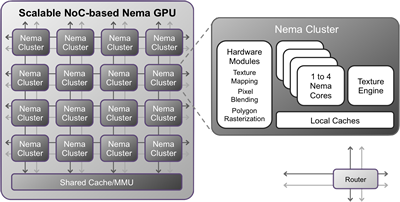
\includegraphics[width=75mm]{figures/nema_diagram}
    \caption{Nema GPU architecture \cite{_nema|s}.}
    \label{fig:nemaarch}
\end{figure}

The implementation of the system is done in zc706 evaluation board from Xilinx. The eGPU is deployed in the FPGA of the Zync7000 processor. The implementation of Nema in this thesis involves 4 cores with 16 threads each. The cores together have a common data cache of 1 MB. The threads are 32 bit. Nema implemented on Zynq 7000 runs with a frequency of 83 MHz.

%


%%%%%%%%%%%%%%%%%%%%%%%%%%%%%%%%%%%%%
%%%%%%%%%%%%%%%%%%%%%%%%%%%%%%%%%%%%%
%%%%%%%%%%%%   SECTION   %%%%%%%%%%%%
%%%%%%%%%%%%%%%%%%%%%%%%%%%%%%%%%%%%%
%%%%%%%%%%%%%%%%%%%%%%%%%%%%%%%%%%%%%
\section{GPU software}
\label{s:gpusw}

GPUs use SIMD (single instruction multiple data) model of programming. They execute the same instructions on different data. The large data set on which the GPU operates is called the stream \cite{Rege}. The set of instructions which operate on each datum is called kernel or shader \cite{Rege}. Each instance of the kernel on a particular ALU is called the thread.

The term shader is used to refer to a kernel as traditionally GPUs were employed for graphic applications. A common application is to render a complete object taking a set of its vertices as inputs. The components of GPU programming are named after the components in graphic rendering. The main parts of GPU programming include blender, rasterizer and interpolators. The blender takes care of the shading environment, like the physical address of the frame buffer (monitor), the colour mode of the shading and the viewport of the image. Rasterizer is responsible for discretising the portions of the object for rendering. For example the object can be a sphere, which is a continuous set of points. However the display environment consists of pixels, a discrete set of points. Rasterizer takes care of the discretization of the sphere so that it can be displayed as an image. A general case is that each thread in a GPU is responsible for each pixel in an image. Hence rasterizer's function can be considered as the deployment of threads in the GPU. Interpolator traditionally is responsible for calculating the colour at a coordinate discretized by rasterizer based on colour at known vertices. In this thesis interpolators are used to calculate the memory locations of the input pixels. The general function of rasterizer and interpolator is as illustrated in the Figure \ref{fig:rastint}.

\begin{figure}
    \center
    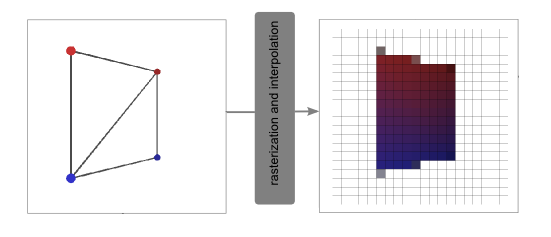
\includegraphics[width=.8\linewidth]{figures/rastint}
    \caption{Function of Rasterizer and Interpolator \cite{Colubri}.}
    \label{fig:rastint}
\end{figure}

%%%%%%%%%%%%%%%%%%%%%%%%%
%%%%%   SUB-SECTION   %%%
%%%%%%%%%%%%%%%%%%%%%%%%%
%%%%%%%%%%%%%%%%%%%%%%%%%
\subsection{Programming Nema}
\label{s:gpusw:nema}

The programming of Nema GPU is done by writing to hardware registers \cite{Apostolou2015}. The values in these register control the workflow of Nema. In C\textbackslash C++Access to these registers is provided by libNemaUtils.so library. The library includes functions to read\textbackslash write to registers and synchronization functions. Like every other C++ library, the libNemaUtils.so needs to be linked with the corresponding header files included for proper function of the host code. The method used for programming Nema is command list method. Commands list consists of a batch of register writes which correspondingly programs the GPU components like blender and rasterizer. Once the command list is ready, it is flushed to the GPU. While the GPU performs the tasks defined by the command list the CPU can continue preparing new command list.

Nema operates on contiguous memory locations. The blender and rasterizer of Nema usually are programmed once for an application. The programming parameters of the blender include starting address, frame buffer stride, frame buffer resolution, viewport and blending mode. The rasterizer is responsible for generating the threads in the GPU. The parameters of Rasterizer include the coordinates of the starting and the ending thread.

Nema includes interpolators that can be programmed to generate values according to the thread coordinates. There are four interpolators available in Nema. Each can be programmed with a starting value step and stride. The values then generated in each GPU thread can be used by the thread for coordinate specific operations. For example, the memory locations of the pixel in the images can be generated by interpolators. Nema also includes constant registers to store the values which remain constant across all GPU threads.The memory space of Nema is managed by nema\_malloc() function. This uses Nema's custom memory manager to ensure that contiguous memory locations are allocated for proper functionality of Nema. The functionality of nema\_malloc() is very similar to that of standard malloc() function. This operates on virtual memory addresses. While transferring the memory location to Nema it needs to be converted to physical address.

nema\_wait\_for\_status() and nema\_wait\_for\_interrupt() are used for synchronization between the host cpu and the gpu. The first functions performs a busy wait polling on the gpu's status register checking if the GPU has completed operation. The second function puts the calling process into a sleep state until the gpu
 raises an interrupt.

%%%%%%%%%%%%%%%%%%%%%%%%%
%%%%%   SUB-SECTION   %%%
%%%%%%%%%%%%%%%%%%%%%%%%%
%%%%%%%%%%%%%%%%%%%%%%%%%
\subsection{Nema kernels}
\label{s:gpusw:nkernels}

 Parallelisable part of the code are written as C kernels in Nema. Each kernel in Nema has access to the interpolater values to perform the particular thread dependent operations. The thread also has access to it's coordinates. Nema also has 16 constant vector registers, meaning 16 registers with 4 32bit element each. An example of kernel is shown in the Appendix \ref{s:kerero}. The read\_reg() function is used to read the constant and interpolator values by each instance of the kernel. The read\_coords() function provides the coordinates of the particular instance of the kernel. These values serve as inputs and outputs for the kernel instance. The kernels are compiled by custom script from ThinkSilicon to generate a .bin file. This .bin file is then loaded into the Nema by the host program during run-time. An example of the host program is provided in the Appendix \ref{s:hostero}. Nema kernels do not have synchronization facilities between the cores. This implies that the threads run independent of each other. Simplified programming structure of Nema eGPU is shown in the Figure \ref{fig:kernelstruct}. The figure indicates the program and data flow between the host and the device (eGPU).

 \begin{figure}
    \center
    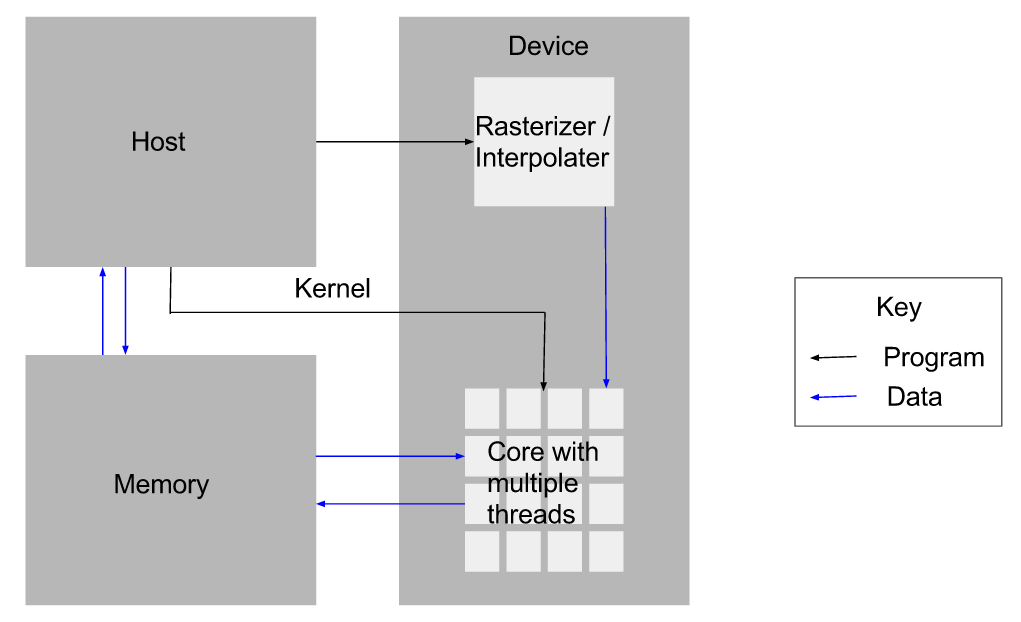
\includegraphics[width=.8\linewidth]{figures/kernelstruct}
    \caption{Simplified program structure in Nema eGPU.}
    \label{fig:kernelstruct}
\end{figure}

%%%%%%%%%%%%%%%%%%%%%%%%%%%%%%%%%%%%%
%%%%%%%%%%%%%%%%%%%%%%%%%%%%%%%%%%%%%
%%%%%%%%%%%%   SECTION   %%%%%%%%%%%%
%%%%%%%%%%%%%%%%%%%%%%%%%%%%%%%%%%%%%
%%%%%%%%%%%%%%%%%%%%%%%%%%%%%%%%%%%%%
\section{Related work}
\label{s:rwork}
A lot of research is done in Stereo vision involving GPUs. GPUs serve as a reliable parallel platform for algorithms such as Stereo vision. They have a fixed architecture and are not limited by space constraints in contrast to FPGAs \cite{Kalarot2010}. In this section some of research done regarding Stereo vision implementation in GPUs are discussed.\\

In \cite{Xu2014}, T. Xu et al. present accelerated version of a Stereo vision algorithm for multi-core CPU and GPU. The evaluated algorithm, the Parallel Pyramid Matcher algorithm, finds application in clothes folding robot. The algorithm is broken down into several subatomic algorithm to understand the performance acceleration. The single core Java implementation (Single Instruction Single Data (SISD)) is compared against Vector Pascal (multi-core) and C\textbackslash C++ \& CUDA implementation (GPU). The experiments were conducted in three different multi-core architectures; AMD Opteron 6366HE, Intel Xeon E5-2440, and Intel Xeon E5-2620; and Nvidia GeForce GTX 770 GPU. One of the interesting findings in the experiment shows a slight increase in execution time of the algorithm in 64 core AMD architecture when the number of threads go beyond 30. This is in contrast with Amdahl's law which expects the execution time to keep decreasing with increase in number of threads provided there is hardware support. The observation is explained by increase in allocation time for threads as the number of used cores increases. Experiments further revealed a 12x speed up in multi-core architecture and 176x speed up with GPU compared to the SISD implementation. The sub-algorithm providing the maximum speed-up was also identified.

Y. Choi et al. propose Graph Cut (GC) based on GPUs for Stereo matching \cite{Choi2013}. The problem of DM creation was approched as a directed graph problem. The method used by Kolmogorov \cite{Kolmogorov2004} is used to construct graphs. Stereo matching is modelled as a multi-label graph problem and is broken down into a series of bi-label problems. Then each bi-label problem is solved using GC. The algorithm is modified to minimized the kernel loading overhead, and to increase the number of computations for global to shared memory transfer in the GPU. Experiments show that 5.2X speedup is obtained in execution time with 0.12\% degradation in accuracy compared to conventional GPU implementation.

Acceleration of SymStereo algorithm using GPU was experimented in \cite{Mota2014}. Unlike conventional Stereo matching algorithms, SymStereo algorithm uses symmetry to evaluate the likelihood of two pixels matching. Generally, Stereo matching can be divided into two parts: creating a disparity space image (DSI) using matching cost functions, and evaluation of DSI to create depth maps. In this paper V. Mota et al. work on accelerating the creation of DSI. Experiments were done on Nvidia Geforce GTX 680 GPU using CUDA 5.0. Across parameters of the algorithm, it was found that they were able to process low-resolution images 53 fps and high-resolution images in 3 fps.

A comparison of FPGA and GPU implementation of real-time Stereo vision was done in \cite{Kalarot2010}. Symmetric Dynamic Programming Stereo (SDPS) is used for the comparison in this paper. Unlike conventional Stereo matching algorithms which create DMs for the right or the left image, SDPS creates a DM for a virtual camera midway between the two cameras. The algorithm is modified to fit the architecture of Altera Stratix III FPGA and Nvidia GTX 280 GPU. It was found that despite a lower clocking rate of the FPGA, it was superior in performance compared to the GPU. The speed-up of FPGA is accounted to the deep extensive pipeline which enables transfer of results from the intermediate stages immediately. The slowdown of GPU was accounted to its internal overheads. It was found however that the bus input\textbackslash output time in the GPU was not a significant contributor to the execution time. It was also found that the FPGA has space limitations with increasing disparity ranges for SDPS algorithm.

\subsection{Summary}
\label{s:rwork:summary}
Intensive research is being done on Stereo vision systems. The focus of the research lies in increasing the accuracy of the system while minimising the execution time. GPUs are evolving as popular implementation platforms for Stereo vision systems. The simpler programming model of GPUs favours them over FPGAs. Algorithms are continually being modified to fit the GPU architecture without sacrificing much of the accuracy of the system. Current research work mostly involves conventional GPUs with a large number of cores. It would be insightful to implement and evaluate a Stereo vision system on an embedded GPU.